\documentclass[../../main.tex]{subfiles}
\graphicspath{{../../image/}{../../figure/}}
\begin{document}

\section{多维标量守恒律的自相似解}\label{section:ch18-多维标量自相似}

我们考虑二维空间中的标量守恒律
\begin{align}
\partial_t u+\partial_x f(u)+\partial_y g(u)=0,
\label{align:ch18-1811}
\end{align}
并寻求自相似解 $u(x,y,t)=v(x/t,y/t)$。令 $\xi=x/t$，$\zeta=y/t$，则 $v(\xi,\zeta)$ 满足方程
\begin{align}
-\xi v_\xi+f(v)_\xi-\zeta v_\zeta+g(v)_\zeta=0.
\label{align:ch18-1812}
\end{align}
\eqref{align:ch18-1812} 的特征线（沿其 $v$ 为常数）由常微分方程确定
\begin{align}
\bigl[f'(v(\xi,\zeta))-\xi\bigr]\,\mathrm{d}\zeta-\bigl[g'(v(\xi,\zeta))-\zeta\bigr]\,\mathrm{d}\xi=0.
\label{align:ch18-1813}
\end{align}
注意奇点集
\begin{align}
\mathscr{B}=\{(\xi,\zeta):\ \xi=f'(v),\ \zeta=g'(v)\},
\label{align:ch18-1814}
\end{align}
它以 $v$ 为参数。为简单起见，我们作假设
\begin{align}
f''(u)>0,\qquad g''(u)>0,\qquad \bigl[f''(u)/g''(u)\bigr]'>0,
\label{align:ch18-1815}
\end{align}
此时 $\mathscr{B}$ 是一条严格递增、凹的曲线 $\zeta=\zeta(\xi)$。

跨越激波曲线的 Rankine--Hugoniot 跳跃条件为
\begin{align}
\bigl[\lambda(u_-,u_+)-\xi\bigr]\,\mathrm{d}\zeta-\bigl[\mu(u_-,u_+)-\zeta\bigr]\,\mathrm{d}\xi=0,
\label{align:ch18-1816}
\end{align}
其中
\begin{align}
\lambda(u_-,u_+)=\frac{f(u_+)-f(u_-)}{u_+-u_-},\qquad
\mu(u_-,u_+)=\frac{g(u_+)-g(u_-)}{u_+-u_-}.
\label{align:ch18-1817}
\end{align}
注意：连接两个固定状态 $u_-$ 与 $u_+$ 的任一激波曲线都落在从节点 $\xi=\lambda(u_-,u_+)$，$\zeta=\mu(u_-,u_+)$ 发出的某条直线上。约定法向量 $(d\zeta,-d\xi)$ 指向激波曲线的 $(+)$ 侧，则可容激波应满足 Oleinik 的 $E$-条件，即
\begin{align}
\bigl[\lambda(u_-,u_0)-\lambda(u_-,u_+)\bigr]\,\mathrm{d}\zeta-\bigl[\mu(u_-,u_0)-\mu(u_-,u_+)\bigr]\,\mathrm{d}\xi\geqslant 0,
\label{align:ch18-1818}
\end{align}
其中 $u_0$ 为介于 $u_-$ 与 $u_+$ 之间的任意状态。

目标是在 $\mathbb{R}^2$ 上构造\eqref{align:ch18-1812}的 $BV$ 解，使其在无穷远处满足给定边界条件：当 $r\to\infty$ 时 $v(r\cos\theta,r\sin\theta)\to h(\theta)$。特别地，经典 Riemann 问题向二维空间的一个自然推广，是确定\eqref{align:ch18-1811}以初始数据
\begin{align}
u(x,y,0)=
\begin{cases}
u_{NE}, & 0<x<\infty,\quad 0<y<\infty\\
u_{SE}, & 0<x<\infty,\quad -\infty<y<0\\
u_{NW}, & -\infty<x<0,\quad 0<y<\infty\\
u_{SW}, & -\infty<x<0,\quad -\infty<y<0,
\end{cases}
\label{align:ch18-1819}
\end{align}
为初始值的自相似解，其中 $u_{NE},u_{SE},u_{NW}$ 与 $u_{SW}$ 为给定常数。

若 $u=v(x/t,y/t)$ 是\eqref{align:ch18-1811}、\eqref{align:ch18-1819}的解，则当 $\xi$（或 $-\xi$）很大时，$v$ 只依赖于 $\zeta$，描绘出一道沿 $y$ 方向传播、连接状态 $u_{NE}$ 与 $u_{SE}$（或 $u_{SW}$ 与 $u_{NW}$）的可容激波或稀疏波。类似地，当 $\zeta$（或 $-\zeta$）很大时，$v$ 只依赖于 $\xi$，描绘出一道沿 $x$ 方向传播、连接状态 $u_{NW}$ 与 $u_{NE}$（或 $u_{SW}$ 与 $u_{SE}$）的可容激波或稀疏波。在 $\xi$-$\zeta$ 平面中上述四道波相互作用的区域，会出现饶有兴味的波型。事实上，依 $u_{NE},u_{SE},u_{NW}$ 与 $u_{SW}$ 在实轴上的相对位置而定，共有 $32$ 种不同的波型构型，它们已在\cref{section:ch18-注记}所引文献中得到描述与分类。为说明起见，下面记录最简单的两种情形。

先设
\begin{align*}
u_{SW}<u_{NW}<u_{SE}<u_{NE}.
\end{align*}
此时解在 $\mathbb{R}^2$ 上 Lipschitz 连续，其等值线如图\cref{figure:ch18-标量扇形波}所示。事实上，状态对 $(u_{NW},u_{NE})$、$(u_{SW},u_{SE})$、$(u_{NE},u_{SE})$ 与 $(u_{NW},u_{SW})$ 均由稀疏波连接。由\eqref{align:ch18-1814}定义的奇点线 $\mathscr{B}$ 标出这些稀疏波之间的边界，并充当一道“脊谷”，使解可跨过它作 Lipschitz 连续过渡。

\begin{figure}[ht]
\centering
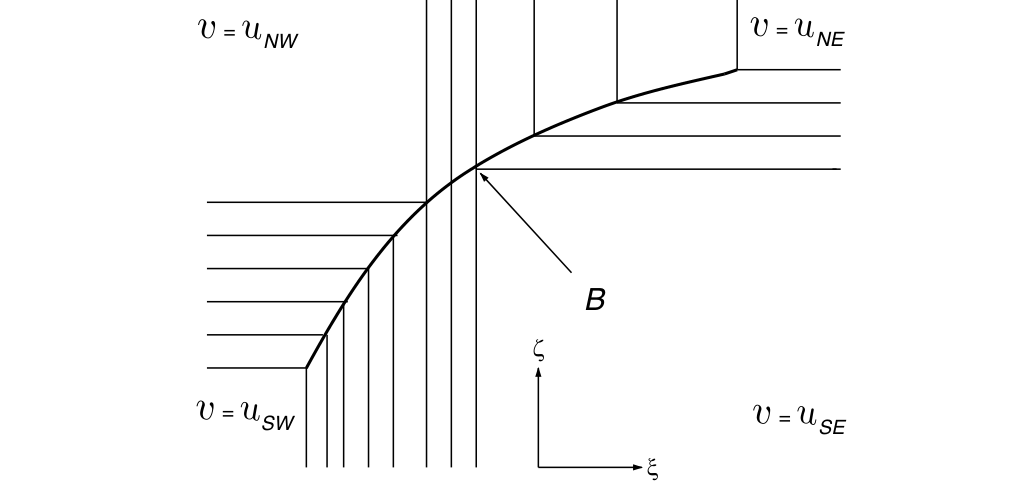
\includegraphics[width=0.72\textwidth]{ch18-fig01-01.png}
\caption{自相似平面中连接四常状态的稀疏波扇形，奇点线 $\mathscr{B}$ 记为 $B$。}
\label{figure:ch18-标量扇形波}
\end{figure}

再设
\begin{align*}
u_{SW}>u_{SE}>u_{NW}>u_{NE}.
\end{align*}
此时解由以可容激波连接的常状态组成，如图\cref{figure:ch18-标量激波构型}所示。事实上，状态对 $(u_{NW},u_{NE})$ 与 $(u_{NW},u_{SW})$ 由两道激波连接，二者在点 $A=(\lambda(u_{NE},u_{NW}),\mu(u_{NW},u_{SW}))$ 相撞；状态对 $(u_{SW},u_{SE})$ 与 $(u_{SE},u_{NE})$ 类似地由两道激波连接，二者在点 $B=(\lambda(u_{SW},u_{SE}),\mu(u_{NE},u_{SE}))$ 相撞。波型由连接 $u_{NE}$ 与 $u_{SW}$ 的两道激波补全：二者均从节点 $O=(\lambda(u_{NE},u_{SW}),\mu(u_{NE},u_{SW}))$ 发出，一道止于点 $A$，另一道止于点 $B$。

\begin{figure}[ht]
\centering
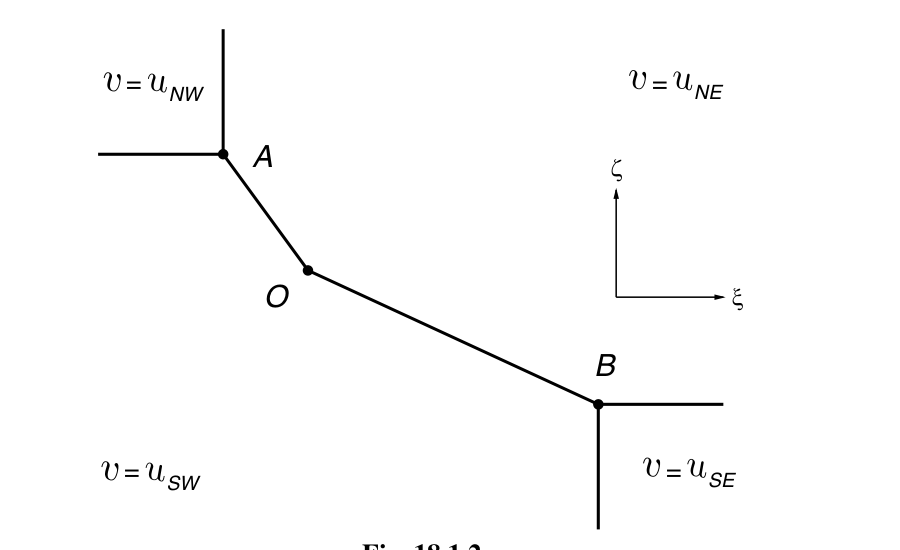
\includegraphics[width=0.72\textwidth]{ch18-fig01-02.png}
\caption{四常状态由激波连接的构型：两道激波分别在 $A$、$B$ 相撞，并自节点 $O$ 发出。}
\label{figure:ch18-标量激波构型}
\end{figure}

其余情形涉及激波与稀疏波的组合，它们可能相互作用而生成更复杂的波型。在缺少\eqref{align:ch18-1815}这类条件时，波型还要更加错综复杂。参见\cref{section:ch18-注记}所引文献。

不必指望多维 Riemann 问题能起到其一维对应物那样关键的作用；尽管如此，它们仍有价值，因为它们直观地展示了多维空间中守恒律方程组解的几何复杂性。

\end{document}
